\documentclass[usepdftitle=false]{beamer}

\usepackage[utf8]{inputenc}
\usepackage{listings}
\usepackage[dvipsnames]{xcolor}
\usepackage{graphicx} % Required for inserting images

\usetheme{Madrid}
\usecolortheme{seahorse}

% Python listing styling
\DeclareFixedFont{\ttb}{T1}{txtt}{bx}{n}{10} % for bold
\DeclareFixedFont{\ttm}{T1}{txtt}{m}{n}{10}  % for normal
\newcommand\pythonstyle{\lstset{
language=Python,
morekeywords={assert},                % Add keywords here
basicstyle=\small\ttm,
keywordstyle=\ttb\color{Green},
emphstyle=\ttb\color{Green},    % Custom highlighting style
stringstyle=\color{OliveGreen},
commentstyle=\color{lightgray},
frame=none,                     % Any extra options here
showstringspaces=false
}}

% Python listing env
\lstnewenvironment{python}[1][]
{
\pythonstyle
\lstset{#1}
}
{}

\title{CRYPTO project SW6}
\author{Alexandru Gabriel Bradatan - 10658858}
\date{December, 2024}

\begin{document}

\frame{\titlepage}

\begin{frame}{Contents}
\tableofcontents
\end{frame}

\section{Background}
\begin{frame}{Project goals}
Our aim is to implement two RSA key-recovery attacks outlined in sections 4.2.7 and 4.2.9 of 
our reference paper \cite{CiC-1-1-28}.

We will try to:
\begin{itemize}
    \item Recover the CRT coefficient $d_p$ from a large known contiguous chunk
    \item Recover one of the primes $p$ from a large known contiguous chunk of the private 
          exponent $d$
\end{itemize}

The code is implemented in a Jupyter Notebook using SageMath version 10.4.
\end{frame}

\subsection{Mathematical Background}
\begin{frame}{Lattices}
Both of our algorithms will make use of lattices and lattice algorithms, so it might be
worthwhile to introduce them a bit.

\begin{definition}
    A lattice $L(B)$, generated by matrix $B\in Mat(n, n, \mathbb{Z})$ with linearly independent
    rows, consists in the integer linear combinations of all rows of $B$.
\end{definition}
\begin{definition}
    The determinant of a lattice is the absolute value of the determinant of a basis matrix:
    \begin{equation}
    \det L(B) = |\det B|
    \end{equation}
\end{definition}
\end{frame}
\begin{frame}{Shortest vector}
\begin{definition}
    In a lattice there will always be a shortest vector $v_1$, which is a vector with the smallest
    non-infinitesimal length in the lattice.
\end{definition}

For a random lattice, we can approximate the length of the shortest vector with the Gaussian
heuristic:
\begin{equation}
\|v_1\|_2 \approx \sqrt{\frac{n}{2 \pi e}}(\det L)^{1/n}
\end{equation}

Since we won't need this much precision and we won't be using large lattices in our work, we will
use this simpler approximation:
\begin{equation}
\|v_1\|_2 \approx (\det L)^{1/n}\label{shortest_vector_len_approx}
\end{equation}
\end{frame}
\begin{frame}{LLL}
\begin{itemize}
    \item The shortest vector in an arbitrary lattice is NP-hard to compute exactly
    \item The LLL algorithm will compute an exponential approximation to this shortest vector
          in polynomial time
    \item In the worst case, the calculated vector $b_1$ will be such that:
    \begin{equation}
        \|b_1\|_2 \leq 2^{\frac{n-1}{4}}(\det L)^{1/n}
    \end{equation}
    \item In practice, for random lattices the bound is tighter:
    \begin{equation}
        \|b_1\|_2 \leq 1.02^n(\det L)^{1/n}
    \end{equation}
\end{itemize}

For our cases, we will need only the fact that vectors returned by LLL will be guaranteed to
be very short.
\end{frame}

\subsection{Cryptographic Background}
\begin{frame}{Quick refresher on RSA}
Let use recap the basic facts about RSA that we will need in our algorithms.

To generate an RSA key-pair:
\begin{enumerate}
    \item Choose a public exponent $e$, in our case $e = 65537$ like $99.\bar{9}\%$ of RSA 
          implementations
    \item Generate two random primes $p, q : gcd(e, (p-1)(q-1)) = 1$
    \item Compute $N = pq$ and $d = e^{-1} \mod (p-1)(q-1)$
\end{enumerate}

Our public key will be $(N, e)$, while the private one will be $(d, N)$.

\vspace{10pt}

To speed up decryption, implementations often use the Chinese Remainder Theorem. This 
optimization splits $d$ into $d_p = d \mod p-1$ and $d_q = d \mod q-1$. The private key in this 
case will be $(d_p, d_q, N)$.
\end{frame}

\section{Recovering $d_p$ from a large contiguous chunk}
\begin{frame}{Overview}
Our first attack consists of recovering the CRT coefficient $d_p$ with knowledge
of a large contiguous part of it. No other knowledge about the private key is assumed.
\vspace{10pt}

There are 3 cases to consider:
\begin{enumerate}
    \item Known most significant bits
    \item Known least significant bits
    \item Known middle bits
\end{enumerate}

We will see all three cases.
\end{frame}

\subsection{Recovery from known MSBs}
\begin{frame}{Recovery from known MSBs: theory}\label{427_msb_alg}
We start from the relation $e d_p \equiv 1 \mod p-1$. We can remove the modulus by 
introducing a new integer variable $k_p$:
\begin{equation}
e d_p = 1 + k_p (p-1) \label{edp_eq}
\end{equation}

Since $d_p < p-1$, we know that $k_p < e$. Since in our case we have a small public
exponent ($e = 65537$), we can brute-force $k_p$:
\begin{itemize}
    \item With the correct parameters, we are guaranteed to find a solution
    \item For incorrect guesses of $k_p$, the attack is unlikely to result in solutions.
          Spurious solutions can be eliminated because they won't factor $N$
\end{itemize}

Rearranging equation~\ref{edp_eq}, with $e^{-1}$ computed modulo $N$, we get:
\begin{align}
    e(a+r) - 1 + k_p        &\equiv 0 \mod p \\
    a + r + e^{-1}(k_p - 1) &\equiv 0 \mod p\label{427_eqn}
\end{align}

Then we apply the algorithm in section 4.2.2.
\end{frame}
\begin{frame}{Recovery from known MSBs: theory}\label{422_alg}
Let $A = a + e^{-1}(k_p - 1)$ and $f(x) = A + x$. We know that $\exists r: f(r) \equiv 0 \mod p$,
$p$ unknown. We know that $|r| < R$ for some bound $R$ that is known. To find $r$:
\begin{enumerate}
    \item Construct the following lattice basis:
            \begin{equation}\label{422_lattice}
                B = \begin{bmatrix}
                    R^2 & RA & 0 \\
                    0   & R  & A \\
                    0   & 0  & N
                \end{bmatrix}
            \end{equation}
          and apply the LLL algorithm to reduce it. Take the shortest vector of the reduced
          basis $v = (v_2 R^2, v_1 R, v_0)$.
    \item Extract the polynomial $f(x) = v_2 x^2 + v_1 x + v_0$ and calculate its roots.
          If any exist, let $r$ be one of them. Verify that $gcd(A + r, N) \neq 1$, 
          in that case $r$ is our unknown chunk, otherwise start again with another $k_p$.
\end{enumerate}
\end{frame}
\begin{frame}{Recovery from known MSBs: more detailed explanation}\label{422_explanation}
\begin{itemize}
    \item The rows of~\ref{422_lattice} correspond to the coefficients of $g_0 = x(x+a)$, $g_1 = x+a$,
          $g_2 = N$. Since $g_n(r) \equiv 0$, then $g|_v(r) \equiv 0 \;\forall v\in L$ mod $p$.
    \item Each column of~\ref{422_lattice} is scaled by a power of $R$, meaning $|g|_v(r)| < \|v\|_1$
          $\forall v\in L$. If $\exists v\in L: \|v\|_2 < p$, then $g|_v(r) < p \land g|_v(r) = 0 \mod p$,
          meaning $g|_v(r) = 0$ over $\mathbb{Z}$.
    \item Using~\ref{shortest_vector_len_approx}, we can obtain the following bound:
        $$
        (\det B)^{1/dim L} = (R^3 N)^{1/3} < p
        $$
    \item  Solving for $R$ and considering that $p\approx N^{1/2}$, we have:
        $$
        R < N^{1/6}
        $$
\end{itemize}

By using bigger lattices and higher order polynomials, this bound can be pushed to $R < N^{1/4}$.
\end{frame}

\begin{frame}[fragile=singleslide]{Recovery from known MSBs: implementation}
The main algorithm outlined in slide~\ref{427_msb_alg} is implemented by the 
\texttt{reconstruct\_dp\_lsb()} function, while the supporting lattice algorithm outlined in
slide~\ref{422_alg} is implemented in \texttt{try\_extract\_lsb\_with\_lattice()}.
\end{frame}

\begin{frame}[fragile=singleslide]{Recovery from known MSBs: code}
\begin{python}
def reconstruct_dp_lsb(rsa, a, l, premul=1,
                       first_kp=1, last_kp=RSA.e):
  inv_e = rsa.e.inverse_mod(rsa.n)
  for kp in range(first_kp, last_kp):
    A = a + inv_e * (kp - 1)
    A *= premul
    res = try_extract_lsb_with_lattice(rsa, A, l)
    if type(res) == Result:
      r = res.unwrap()
      sum = A + r * premul.inverse_mod(rsa.n)
      p = gcd(sum, rsa.n)
      if gcd(p, rsa.n) == p:
        return Result((kp, r))
  return Err(...)
\end{python}
\end{frame}
\begin{frame}[fragile=singleslide]{Recovery from known MSBs: code}
\begin{python}
def try_extract_lsb_with_lattice(rsa, A, l):
  assert l < rsa.bit_length // 6
  R = 2**l
  P.<X> = PolynomialRing(ZZ)
  # --- snip: lattice basis ---
  B = B.LLL()
  v = B[0].list()
  v[0] = v[0] >> l*2
  v[1] = v[1] >> l
  f = v[0] * (X**2) + v[1] * X + v[2]
  roots = f.roots()
  for root in roots:
    r = Integer(root[0])
    if gcd(A + r, rsa.n) != 1:
      return Result(r)
  return Err("...")
\end{python}
\end{frame}
\begin{frame}{Recovery from known MSBs: parallelization}
Due to the fact that we are brute-forcing the value of $k_p$, we can optimize performance a little
by applying some coarse-grain parallelism, allowing to reduce execution time from $\approx 6$s to
$\approx 1.5$s for an example 240-bit key on a Ryzen 5700U laptop with 16Gb of RAM.

\vspace{10pt}

The scheduling algorithm is implemented by \texttt{schedule\_block()}, while the multi-processed
version of the function is implemented by \texttt{reconstruct\_dp\_lsb\_mp()}.
\end{frame}

\subsection{Recovery from known LSBs}
\begin{frame}{Recovery from known LSBs: theory}\label{427_lsb_alg}
We can reuse the same algorithm we defined before, but apply the tweak described in section 4.2.3.
\vspace{10pt}

Let $l$ be the starting point of the unknown chunk.
\begin{enumerate}
    \item Repeat the same calculations as in slide~\ref{427_msb_alg} to obtain the polynomial
          $f(x) = 2^l x + A$.
    \item We multiply both sides of~\ref{427_eqn} by $2^{-l} \mod N$ to obtain the same polynomial
          as in slide~\ref{422_alg}.
    \item Proceed with the same algorithm as slide~\ref{422_alg}.
    \item After we have solved for $r$ we multiply it by $2^l \mod N$ and obtain the unknown MSBs.
\end{enumerate}

Since we are reusing the algorithm in~\ref{427_msb_alg}, we have that this method will work knowing as
few as $N^{1/6}$ LSBs of $d_p$, $N^{1/4}$ at the limit.
\end{frame}
\begin{frame}{Recovery from known LSBs: implementation}
The implementation reuses the previously defined \texttt{reconstruct\_dp\_lsb()} and 
\texttt{reconstruct\_dp\_lsb\_mp()}, using the purposely defined optional parameter \texttt{premul}
to multiply $A$ by $2^{-l} \mod N$ before the call to \texttt{try\_extract\_lsb\_with\_lattice()}.
Then it simply unpacks the result and multiplies it by $2^l$ before returning it.

\vspace{10pt}

Since we are reusing the same methods as before with minimal changes, the same considerations apply.
\end{frame}
\begin{frame}[fragile=singleslide]{Recovery from known LSBs: code}
\begin{python}
def reconstruct_dp_msb_mp(rsa, a, m):
  assert m > rsa.bit_length // 6
  l = rsa.bit_length//2 - m
  R = 2**m
  mul = R.inverse_mod(rsa.n)
  kp, r = reconstruct_dp_lsb_mp(rsa, a, l,
                                premul=mul).unwrap()
  return Result((kp, r * R))
\end{python}
\end{frame}

\subsection{Recovery from known middle bits}
\begin{frame}{Recovery from known middle bits: theory}\label{427_mid_alg}
We can reuse part of the method we devised for recovery from known MSBs,  but apply the algorithm 
outlined in 4.2.4 instead of that in 4.2.2.
\vspace{10pt}

Let $d_p = 2^t r_m + a + r_l$, $a$ the known chunk and $R$ such that $|r_l| < R$ and $|r_m| < R$.
\begin{enumerate}
    \item Apply the same calculations as in slide~\ref{427_msb_alg} for a certain $k_p$ to obtain:
        \begin{align}
            2^t r_m + a + r_l + e^{-1}(k_p - 1) \equiv 0 \mod p \\
            A = a + e^{-1}(k_p - 1) \quad\quad f(x) = 2^t y  + A + x\label{424_poly}
        \end{align}
    \item Reduce the lattice basis outlined in section 4.2.4 using LLL
    \item Extract $f|_v$, $v$ vector of the reduced basis, and find the common roots $x=r_l, y=r_m$ of
          the system using Groebner bases.
    \item If $gcd(A + r_l + r_m, N) \neq 1$, then $r_l$ and $r_m$ are our solutions, otherwise try 
          another $k_p$.
\end{enumerate}
\end{frame}
\begin{frame}{Recovery from middle bits: more detailed explanation}
The reasoning behind this algorithms is largely the same as in slide~\ref{422_explanation}, but with
some slight differences.

\begin{itemize}
    \item We want $v_1, v_2 : \|v_1\|_2 \approx \|v_2\|_2$, but we aren't guaranteed to find them. However,
          for random lattices we expect the lengths of the vectors in the reduced basis to be approximately
          the same. 
    \item Like in slide~\ref{422_explanation}, we will have:
          $$
          |f|_v(r_l, r_m)| < \|v\|_1 < p \approx N^{1/2}
          $$
    \item Thus, using~\ref{shortest_vector_len_approx}, our bound will be:
          $$
          (\det B)^{1/dimL} = (R^{20}N^4)^{1/10} < N^{1/2} 
          $$
    \item Solving for $R$ we get:
          $$
          R^{20} < N
          $$
\end{itemize}
\end{frame}
\begin{frame}[fragile=singleslide]{Recovery from known middle bits: implementation}
The algorithm outlined in slide~\ref{427_mid_alg} is implemented by \texttt{reconstruct\_dp\_mid()},
while the supporting lattice algorithm is implemented by \texttt{try\_extract\_mid\_with\_lattice()}.
Just like the others, it is easily parallelized (implemented in \texttt{reconstruct\_dp\_mid\_mp()}).
\vspace{10pt}

Since this version of the code uses a bigger lattice and does many more calculations, its runtime
increased to $\approx$4 minutes for the same 240-bit modulus.

\begin{alertblock}{Important note}
Another very important reason we parallelize \texttt{reconstruct\_dp\_mid()} is to work around a memory leak
in \texttt{groebner\_basis()}! Being called so frequently ($\approx$650k times!), it can easily exhaust the
host's memory.
\vspace{10pt}

\texttt{schedule\_block\_leaky} is a variant of \texttt{schedule\_block} that closes the \texttt{ProcessPool}
every time a round of workers finishes, allowing the OS to regain the leaked memory and avoid OOM.
\end{alertblock}
\end{frame}
\begin{frame}{Memory leak memory usage}
\begin{figure}
\centering
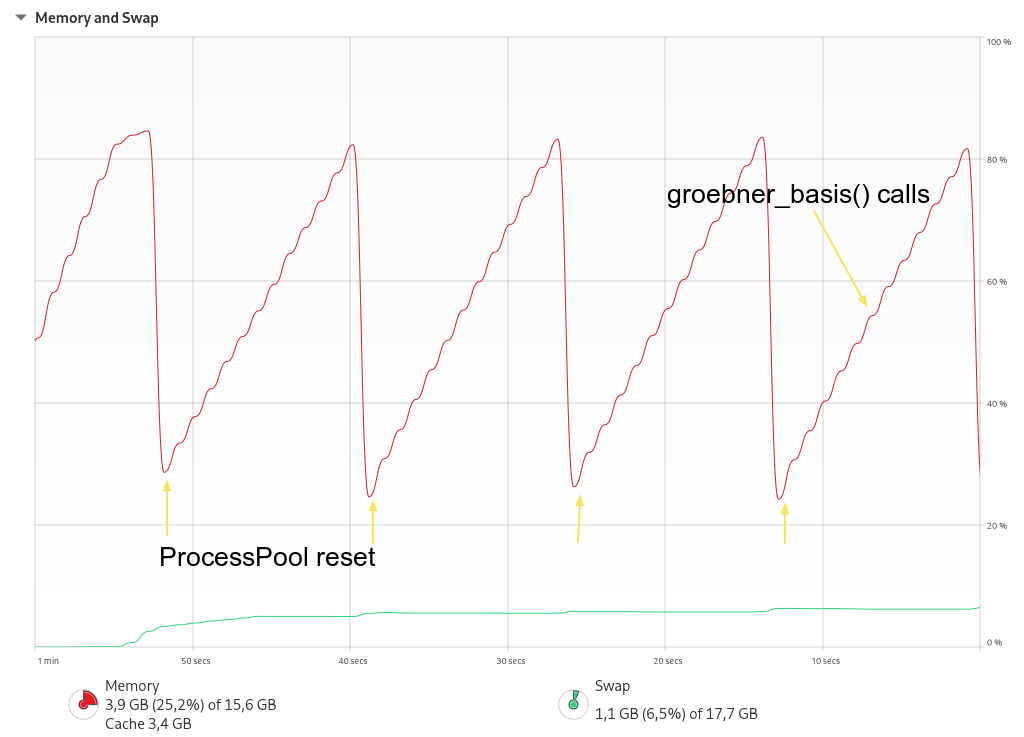
\includegraphics[width=250px]{leaked_mem.png}
\caption{Memory usage during the execution of \texttt{reconstruct\_dp\_mid\_mp()}}
\end{figure}
\end{frame}
\begin{frame}[fragile=singleslide]{Recovery from known middle bits: code}
\begin{python}
def reconstruct_dp_mid(rsa, a, l, m, t,
                       first_kp=1, last_kp=RSA.e):
  exp = max(l, t)
  assert exp*20 < rsa.bit_length
  t_shift = l + m
  inv_e = rsa.e.inverse_mod(rsa.n)
  for kp in range(first_kp, last_kp):
    A = ZZ(mod(a + inv_e * (kp - 1), rsa.n))
    res = try_extract_mid_with_lattice(rsa, A,
                                       t_shift, exp)
    if type(res) == Result:
      rm, rl = res.unwrap()
      return Result((kp, rm, rl))
  return Err("...")
\end{python}
\end{frame}
\begin{frame}[fragile=singleslide]{Recovery from known middle bits: code}
\begin{python}
def try_extract_mid_with_lattice(rsa, A, t, exp):
  # --- snip: some convenience variables ---
  assert exp*20 < rsa.bit_length
  P.<X,Y> = PolynomialRing(ZZ)
  # --- snip: lattice basis definition ---
  B = B.LLL()
  monomials = vector((X^3, X^2*Y, X*Y^2, Y^3,
                      X^2, X*Y, Y^2, X, Y, 1))
  polys = []
  for r in B:
    r[0:4] /= R3
    r[4:7] /= R2
    r[7:9] /= R
    polys.append(r * monomials)
  # --- continued ---
\end{python}
\end{frame}
\begin{frame}[fragile=singleslide]{Recovery from known middle bits: code}
\begin{python}
  # --- try_extract_mid_with_lattice continued ---
  for i in range(2, len(polys)+1):
    gb = ideal(polys[0:i]).groebner_basis()
    if gb[-1].degree() != 1:
      continue
    y_roots = gb[-1].univariate_polynomial().roots()
    if len(y_roots) != 1:
      return Err("...")
    rm = ZZ(y_roots[0][0])
    px = gb[-2].substitute({Y: rm})
    x_roots = px.univariate_polynomial().roots()
    if len(x_roots) != 1:
      return Err("...")
    rl = ZZ(x_roots[0][0])
    return Result((rm, rl))
  return Err("...")
\end{python}
\end{frame}

\section{Recovering $p$ from large contiguous chunks of $d$}
\begin{frame}{Recovery of $p$ from $d$: theory}\label{429_alg}
For low-exponent RSA like our case, if we know the $t$ LSBs of $d$, then we can extrapolate knowledge of
the $t$ LSBs of $p$. Then, to recover the MSBs, we can apply the method of section 4.2.3, which is also the base for the algorithm in~\ref{427_lsb_alg}.
\end{frame}
\begin{frame}{Recovery of $p$ from $d$: theory}
\begin{enumerate}
    \item Let $d_0$ be the known chunk, then we can write:
        $$
        e d_0 \equiv 1 + k(N - (p+q) + 1) \equiv 1 + k(N - s + 1) \mod 2^t 
        $$
        We will brute-force $k$ to obtain candidate values for the LSBs of $s$.
    \item For each candidate $s$, the $t$ LSBs of $p$ are solutions to the following equation
        \begin{equation}
            p^2 - sp + N \equiv 0 \mod 2^t\label{429_quadratic}
        \end{equation}
    \item Let $a$ be a candidate solution to~\ref{429_quadratic}. Similarly to~\ref{427_lsb_alg}, we
          obtain $f(x) = a + 2^t x \equiv 0 \mod p$.
    \item First multiply it by $2^{-t} \mod N$, then apply the algorithm in slide~\ref{422_alg}.
    \item If we have a solution $r$, multiply it by $2^t$ obtaining $p = a + r$.
\end{enumerate}

Since the base method recovers up to $N^{1/6}$ bits of p, this will work knowing as few as $N^{1/6}$ 
LSBs of $d$, at the limit $N^{1/4}$.
\end{frame}
\begin{frame}[fragile=singleslide]{Recovery of $p$ from $d$: implementation}
The algorithm of slide~\ref{429_alg} is implemented by the \texttt{reconstruct\_p()} function and it
uses the already defined \texttt{try\_extract\_lsb\_with\_lattice()} function internally. Since, like
the other attacks in this presentation, we need to bruteforce $k$, we reused the same parallelization 
scheme to gain some performance.
\vspace{10pt}

This algorithm is more computationally intensive than those to recover the MSBs of $d_p$, 
getting $\approx$3 minutes of runtime for a 64-bit modulus, instead of a couple of seconds for
a 240-bit one like before.

\begin{alertblock}{Important note}
Again, like with \texttt{reconstruct\_dp\_mid()}, we have to work around a leak, albeit a much smaller one,
inside \texttt{solve\_mod()}. We used the same \texttt{schedule\_block\_leaky()} as before to do so.
\end{alertblock}
\end{frame}
\begin{frame}[fragile=singleslide]{Recovery of p: code}
\begin{python}
def reconstruct_p(rsa, d0, t, start_k=2, end_k=RSA.e):
  # --- snip: support variables ---
  for k in range(start_k, end_k):
    S_sols = solve_mod(
      rsa.e*d0 == 1 + k*(rsa.n - S + 1), R)
    for s in S_sols:
      s = ZZ(s[0])
      P_sols = solve_mod(P**2 - s * P + rsa.n == 0, R)
      for a in P_sols:
        a = ZZ(a[0])
        A = mul * a
        res = try_extract_lsb_with_lattice(rsa, A, l)
        if type(res) == Result:
          r = gcd(a + res.unwrap() * R, rsa.n)
          return Result(r)
  return Err("...")
\end{python}
\end{frame}

\section{Conclusions}
\begin{frame}{Conclusions}
We have successfully provided proof-of-concept implementations of the algorithms presented in sections
4.2.7 and 4.2.9 of our reference paper, successfully working around the problems encountered with Sage.
\end{frame}

\begin{frame}{References}
\bibliographystyle{plain}
\bibliography{refs}
\end{frame}

\end{document}
